% Created 2022-05-10 Tue 10:37
% Intended LaTeX compiler: pdflatex
\documentclass[smaller]{beamer}\usepackage{listings}
\usepackage{color}
\usepackage{amsmath}
\usepackage{array}
\usepackage[T1]{fontenc}
\usepackage{natbib}
\lstset{
keywordstyle=\color{blue},
commentstyle=\color{red},stringstyle=\color[rgb]{0,.5,0},
literate={~}{$\sim$}{1},
basicstyle=\ttfamily\small,
columns=fullflexible,
breaklines=true,
breakatwhitespace=false,
numbers=left,
numberstyle=\ttfamily\tiny\color{gray},
stepnumber=1,
numbersep=10pt,
backgroundcolor=\color{white},
tabsize=4,
keepspaces=true,
showspaces=false,
showstringspaces=false,
xleftmargin=.23in,
frame=single,
basewidth={0.5em,0.4em},
}
\usepackage{natbib, dsfont, pgfpages, tikz,amssymb, amsmath,xcolor}
\bibliographystyle{abbrvnat}
% New operators and commands
\newcommand{\Z}{\mathbb{Z}}
\newcommand{\Q}{\mathbb{Q}}
\newcommand{\R}{\mathbb{R}}
\newcommand{\N}{\mathbb{N}}
\newcommand{\C}{\mathbb{C}}
\renewcommand{\S}{\mathbb{S}}
\newcommand{\blank}{\makebox[1ex]{\textbf{$\cdot$}}}
\newcommand\independent{\protect\mathpalette{\protect\independenT}{\perp}}
\def\independenT#1#2{\mathrel{\rlap{$#1#2$}\mkern2mu{#1#2}}}
\renewcommand{\phi}{\varphi}
\renewcommand{\epsilon}{\varepsilon}
\newcommand*\diff{\mathop{}\!\mathrm{d}}
\newcommand{\weakly}{\rightsquigarrow}
\newcommand\smallO{
  \mathchoice
    {{\scriptstyle\mathcal{O}}}% \displaystyle
    {{\scriptstyle\mathcal{O}}}% \textstyle
    {{\scriptscriptstyle\mathcal{O}}}% \scriptstyle
    {\scalebox{.6}{$\scriptscriptstyle\mathcal{O}$}}%\scriptscriptstyle
}
\newcommand{\midd}{\; \middle|\;}
\newcommand{\1}{\mathds{1}}
\usepackage{ifthen} %% Empirical process with default argument
% \newcommand{\G}[1][]{%
%    \ifthenelse{ \equal{#1}{} }
%       {\ensuremath{\mathbb{G}_n}}
%       {\ensuremath{\mathbb{G}_{#1}}}
% }
% New version:
\newcommand{\G}[2][n]{
{\ensuremath{\mathbb{G}_{#1}}{\left[#2\right]}}
}
\DeclareMathOperator*{\argmin}{\arg\!\min}

% New operators for consistent notation
\newcommand{\V}{\mathrm{Var}} % variance
\newcommand{\measure}[1]{\mathrm{{#1}}} % measure
% \newcommand{\measure}[1]{\textnormal{\textbf{{#1}}}} % measure
\newcommand{\m}[1]{\measure{#1}} % measure shortcut
\newcommand{\eqd}{\stackrel{d}{=}} % equality in distribution
\newcommand{\arrowP}{\xrightarrow{\; \m{P} \;}} % convergence in probability
\newcommand{\leb}{\lambda} % the Lebesgue measure
\newcommand{\T}{\top} % transpose

\usepackage{xargs}
% Make it easy to change counterfactual notation:
\newcommandx{\cf}[4][3={}, 4={}]{
  % \ifthenelse{ \equal{#4}{} }
  % {{#1^{#2}}(#3)}
  {\ifthenelse{ \equal{#3}{} }
    {{#1^{#2}}_{#4}}
    {{#1^{#2}}_{#4}(#3)}}
}

% Easily change notation:
\DeclareMathOperator{\TT}{\Psi} % target parameter
\newcommand{\lp}{\mathcal{L}_{\P}^2} % shortcut for lp2 space
\newcommand{\empmeas}{\hat{\mathbb{P}}_n} % empirical measure
\DeclareMathOperator{\E}{\mathbb{E}} % expectation
\renewcommand{\P}{\m{P}} % probability
\newcommand{\ic}{\mathrm{IF}} % influence curve
\setbeamertemplate{footline}[frame number]
\beamertemplatenavigationsymbolsempty
\usepackage{appendixnumberbeamer}
\setbeamercolor{gray}{bg=white!90!black}
\setbeamertemplate{itemize items}{$\circ$}
\lstset{basicstyle=\ttfamily\footnotesize}

\renewcommand*\familydefault{\sfdefault}
\itemsep2pt
\usepackage[utf8]{inputenc}
\usepackage[T1]{fontenc}
\usepackage{graphicx}
\usepackage{longtable}
\usepackage{wrapfig}
\usepackage{rotating}
\usepackage[normalem]{ulem}
\usepackage{amsmath}
\usepackage{amssymb}
\usepackage{capt-of}
\usepackage{hyperref}
\usetheme{default}
\author{Anders Munch}
\date{May 10, 2022}
\title{Targeted Learning}
\begin{document}

\maketitle
\begin{frame}[label={sec:orgc6cac3e}]{Scientific parameter of interest}
\small To make sure that our statistical analysis is of any interest, we should make sure that we
estimate a meaningful and clearly interpretable parameter that answers a specific scientific
question.
\begin{exampleblock}{The average treatment effect (ATE)}
Let $\mathcal{P}$ be a collection of probability measures over $\R^{d+2}$, so that
$O \sim P \in \mathcal{P}$, with $O = (Y, A, X)$, $Y\in \R$, $A\in \{0,1\}$, and $X \in
\R^d$. Define
\begin{align*}
  \Psi(P)
  & = \E_P{\left[ \E_P[Y \mid X, A=1] - \E_P[Y \mid X, A=0] \right]} \\
  & = \int {\left\{ \nu_P(x, 1) - \nu_P(x, 0) \right\}} \mu_P(\diff x),
\end{align*}
where $\nu_P$ denotes the conditional expectation of $Y$ given $X$ and $A$, and $\mu_P$ denotes the
marginal distribution of $X$. 
Under suitable structural assumptions \(\Psi(P)\) can be given a causal interpretation, see
\citep{kennedy2016semiparametric,hernanRobinsWhatIf} for more details. In particular, one
assumption is that there is no unmeasured confounding.
\end{exampleblock}
\end{frame}

\begin{frame}[label={sec:orgb7fb5b7}]{Nuisance and target parameters}
To obtain an estimator of \(\Psi(P)\) we can exploit that this parameter is identified through the
parameters \(\nu\) and \(\mu\). With estimator \(\hat\nu_n\) and \(\hat\mu_n\) we obtain the plug-in
estimator
\begin{equation*}
  \hat{\Psi}_n^0 = \int {\left\{ \hat{\nu}_n(x, 1) - \hat{\nu}_n(x, 0) \right\}} \hat{\mu}_n(\diff x).
\end{equation*}
When we use the empirical measure
\begin{equation*}
  \empmeas := \frac{1}{n}\sum_{i=1}^{n}\delta_{O_i},
\end{equation*}
to estimate $\mu$, the estimator $\hat{\Psi}_n$ becomes simply
\begin{equation*}
  \hat{\Psi}_n^0 = \frac{1}{n} \sum_{i=1}^{n} {\left\{ \hat{\nu}_n(X_i, 1) - \hat{\nu}_n(X_i, 0) \right\}}.
\end{equation*}

The parameters \(\nu\) and \(\mu\) are (in this case) not something we are interested in. The only
reason to estimating them is to obtain an estimator of \(\Psi\). Hence \(\nu\) and \(\mu\) are referred to
as \emph{nuisance parameters} while \(\Psi\) is the \emph{target parameter}.
\end{frame}
\begin{frame}[label={sec:org0d29bf7},fragile]{Example with \texttt{R}-code (G-formula)}
 \lstset{language=r,label= ,caption= ,captionpos=b,numbers=none}
\begin{lstlisting}
set.seed(20)
sim.dat <- function(n=1000, p=10){
  X0 = matrix(rnorm(n*p), nrow=n)
  A = 1*(runif(n) < .5)
  Y = A*0.2 + rnorm(n)
  return(data.table(Y, A, X0))
}
dat = sim.dat()
model = cv.glmnet(as.matrix(dat[, -1]), dat[,Y], alpha=0)
dat_c = copy(dat)
dat_c[, A:=0]
fit0 = predict(model, newx=as.matrix(dat_c[, -1]), s = "lambda.min")
dat_c[, A:=1]
fit1 = predict(model, newx=as.matrix(dat_c[, -1]), s = "lambda.min")
mean(fit1 - fit0)
\end{lstlisting}

\begin{verbatim}
[1] 0.06748045
\end{verbatim}
\end{frame}

\begin{frame}[label={sec:org00ae6d9}]{Low and high-dimensional nuisance parameter}
\begin{block}{Low-dimensional nuisance parameters}
In the case that we assume the nuisance parameters to be low-dimensional, for instance
$\mathcal{P} = \{P_{\theta} \; : \; \theta \in \R^3\}$, it would often be straightforward to analyze
the asymptotic behavior of $\Psi(P_{\hat{\theta}_n})$ if we know the asymptotic behaviour of
$\hat{\theta}_n$. \dots \textbf{How?}\pause
\end{block}

\begin{block}{High-dimensional nuisance parameters}
When the nuisance parameter \(\hat\theta_n\) is high-/infinite-dimensional, things become more
complicated:
\begin{enumerate}
\item Often we do not know the asymptotic distribution of \(\hat\theta_n\).
\item Even if we did, this would not help us to a good estimator of \(\Psi(P_{\hat{\theta}_n})\).
\end{enumerate}

\vfill

\dots{} \textbf{Why then bother with high-dimensional nuisance parameters?}
\end{block}
\end{frame}

\begin{frame}[label={sec:orgc58669d}]{The challenge with high-dimensional nuisance parameters}
The nuisance estimators is optimized for minimizing the MSE for the \emph{nuisance} parameter and not for
the \emph{target} parameter.

\begin{center}
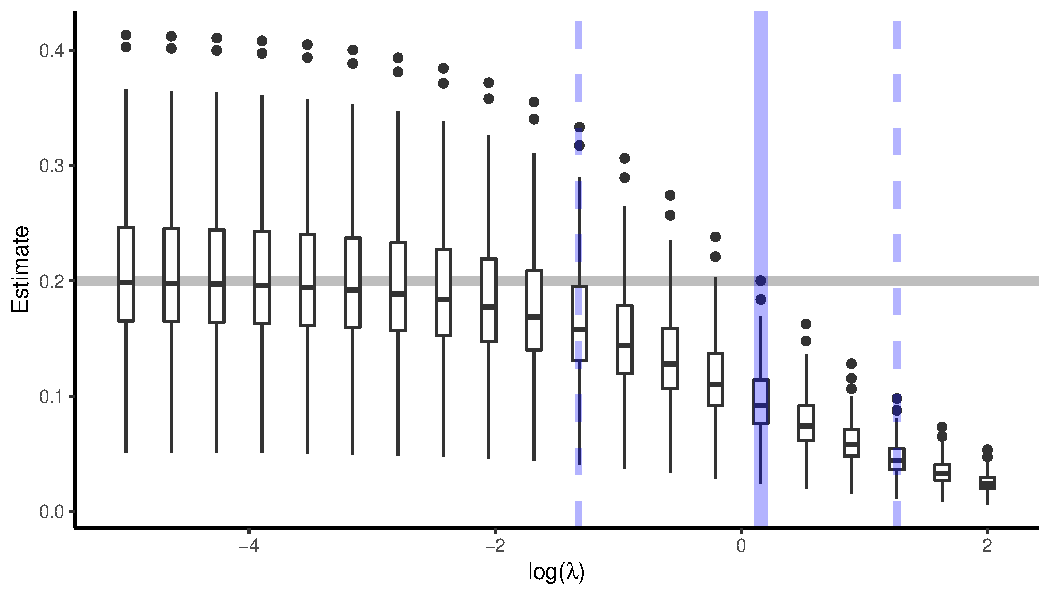
\includegraphics[width=.9\linewidth]{fig-target-hyperpar-effect.pdf}
\end{center}
\end{frame}

\begin{frame}[label={sec:org85d74e0}]{Asymptotic linear estimators}
\small
For a function $f \colon \mathcal{O} \rightarrow \R$ and a measure $P$ on $\mathcal{O}$ we use the notation $P[f]$ to mean
\begin{equation*}
  P[f] := \int f(o)  P(\diff o).
  \quad \text{For example, } \quad
  \empmeas[f] = \frac{1}{n}\sum_{i=1}^{n}f(O_i).
\end{equation*}
We write $X_n = \smallO_P(r_n)$ to mean that $X_n/r_n \arrow{P} 0$. In particular, $\smallO_P(1)$
denotes a term that converges to 0 in probability. 

\begin{definition}[RAL estimators]
An estimator $\hat{\Psi}_n$ of the parameter $\Psi$ under the model $\mathcal{P}$, is
called \textit{asymptotically linear} with \textit{influence function} $\ic(\blank, P)$, if 
$P[\ic(\blank, P)] = 0$ for all $P \in \mathcal{P}$, and 
\begin{equation*}
  \sqrt{n}(\hat{\Psi}_n - \Psi) = \sqrt{n}(\empmeas-P)[\ic(\blank, P)] + \smallO_{P}(1).
\end{equation*}

\vfill

By the central limit theorem
$\sqrt{n}(\hat{\Psi}_n - \Psi) \rightsquigarrow \mathcal{N}(0,  P[\ic(\blank, P)^2])$.

\hfill

The influence function of the RAL estimator with the smallest asymptotic variance is called the
\emph{efficient influence} function or the \emph{canonical gradient}.
\end{definition}
\end{frame}

\begin{frame}[label={sec:org7005a15}]{The asymptotic behavior of \(\hat\Psi_n^0\)}
\small If we make no assumptions\footnote{For estimation to be possible and positivity to hold we end up making \emph{some} assumptions.} about \(\mathcal{P}\) then all RAL estimators of a parameter
\(\Psi\) have the same influence function \citep{kennedy2016semiparametric}. Let \(\ic(\blank;P)\) denote this
unique influence function, and let \(\hat P_n\) denote an estimator of \(P\). Then we may write
\begin{align*}
  & \sqrt{n}(\hat{\Psi}_n^0 - \Psi)
  \\
  & = \sqrt{n}
    \Psi(\hat P_n) - \Psi(P)
  \\
  &  = \sqrt{n}
    \left(
    \Psi(\hat P_n) - \Psi(P)
    \pm
    (\empmeas-P)[\ic(\blank; \hat P_n)]
    \right)
  \\
  &  = \sqrt{n}(\empmeas-P)[\ic(\blank; \hat P_n)]
    - \sqrt{n}\empmeas[\ic(\blank; \hat P_n)]
    + \sqrt{n}\mathrm{Rem}(P,  \hat P_n),
  % & = \sqrt{n}
  %   \left(
  %   \empmeas{[\phi(\blank; \hat{\nu}_n)]} - P{[\phi(\blank; \nu)]}
  %   \right)    
  % \\
  % &  = \sqrt{n}
  %   \left(
  %   \empmeas{[\phi(\blank; \hat{\nu}_n)]} - P{[\phi(\blank; \nu)]} \pm
  %   (\empmeas-P)[\ic(\blank; \hat{\nu}_n, \hat{\pi}_n)]
  %   \right)
  % \\
  % &  = \sqrt{n}(\empmeas-P)[\ic(\blank; \hat{\nu}_n, \hat{\pi}_n)]
  %   - \sqrt{n}\empmeas[\ic(\blank; \hat{\nu}_n, \hat{\pi}_n)]
  %   + \sqrt{n}\mathrm{Rem}(P,  \hat{\nu}_n, \hat{\pi}_n),
\end{align*}
where we define
\begin{equation*}
  \mathrm{Rem}(P,  \hat{P}_n)
  := \Psi(\hat P_n) 
  + P[\ic(\blank; \hat P_n)]
  - \Psi(P).
\end{equation*}
% \begin{equation*}
%   \mathrm{Rem}(P,  \hat{\nu}_n, \hat{\pi}_n)
%   := \empmeas{[\phi(\blank; \hat{\nu}_n)]} - P{[\phi(\blank; \nu)]}
%   + P[\ic(\blank; \hat{\nu}_n, \hat{\pi}_n)].
% \end{equation*}
Here \(\Psi\) and \(\ic\) might depend on different components of the measure \(P\), for instance \(\Psi\)
might depend on the nuisance parameters \(\nu\) and \(\mu\) while \(\ic\) depend on \(\mu\) and \(\pi\).
\end{frame}

\begin{frame}[label={sec:org6a22f23}]{The main variance term and the remainder}
\small
\begin{block}{\((\empmeas-P)[\ic(\blank; \hat{P}_n)]\)}
The first term can be controlled using \emph{empirical process theory} or \emph{sample splitting} (see
\cite{kennedy2022semiparametric}), which allows us to write \[ \sqrt{n}(\empmeas-P)[\ic(\blank;
\hat P_n)] = \sqrt{n}(\empmeas-P)[\ic(\blank; P)] + \smallO_P(1).\]
\end{block}

\begin{block}{\(\mathrm{Rem}(P, \hat{P}_n)\)}
The influence function can also be understood as a \emph{functional derivative} of the parameter
\(\Psi\colon \mathcal{P} \rightarrow \R\). Thus \[\Psi(\hat P_n) + P[\ic(\blank; \hat{P}_n)]\] can be
understood as a first order functional Taylor approximation to \(\Psi(P)\). If \(\| \hat{P}_n -P \| =
\smallO_P(n^{-1/4})\) we might therefore expect that \[ \mathrm{Rem}(P, \hat{P}_n) = \Psi(\hat P_n) +
P[\ic(\blank; \hat{P}_n)] - \Psi(P) = \smallO_P((n^{-1/4})^2) = \smallO_P(n^{-1/2}). \]
\end{block}
\end{frame}

\begin{frame}[label={sec:orgc7cb200}]{One-step / debiased estimator}
\small
Combining these steps gives that
\begin{align*}
  & \sqrt{n}(\hat{\Psi}_n^0 - \Psi) 
  \\
    &  = \sqrt{n}(\empmeas-P)[\ic(\blank; \hat{P}_n)]
    - \sqrt{n}\empmeas[\ic(\blank; \hat{P}_n)]
    + \sqrt{n}\mathrm{Rem}(P,  \hat{P}_n)
    \\
    & =
    \sqrt{n}(\empmeas-P)[\ic(\blank; P)]
    - \sqrt{n}\empmeas[\ic(\blank; \hat{P}_n)]
    + \smallO_P(1).
\end{align*}

When the nuisance parameters \(\nu\) and \(\pi\) are high-dimensional the bias of the estimators
\(\hat{\nu}_n\) and \(\hat{\pi}_n\) are typically larger than \(\sqrt{n}\), and hence the second term
above prevents our estimator from being RAL.

\vfill

A \emph{one-step} or \emph{debiased estimator} handles this problem simply by replacing \(\hat\Psi_n^0\) with
the estimator \[\hat\Psi_n:= \hat\Psi_n^0 + \empmeas[\ic(\blank; \hat{P}_n)],\] as then \[\sqrt n
(\hat\Psi_n - \Psi):= \sqrt{n}(\empmeas-P)[\ic(\blank; P)] + \smallO_P(1),\] i.e., \(\hat\Psi_n\) is
RAL with influence function \(\ic\).
\end{frame}

\begin{frame}[label={sec:org1858cfc}]{The canonical gradient for the ATE}
\small For the ATE problem the canonical gradient is
\begin{align*}
  \ic(O; P)
  & = \nu_P(X, 1) - \nu_P(X, 0)
  \\
  & \quad
    + \frac{A}{\pi_P(X)}(Y - \nu_P(X, 1))
    - \frac{1-A}{1-\pi_P(X)}(Y - \nu_P(X, 0))
  \\
  & \quad
    - \Psi(P),
\end{align*}
where \(\pi\) denotes the \textit{propensity score} \(\pi(x) := P(A=1 \mid X=x)\), see
\cite{kennedy2022semiparametric,kennedy2016semiparametric}.

\vfill

With estimators of \(\nu\) and \(\pi\) the one-step estimator becomes
\begin{align*}
  \hat{\Psi}_n
  &  = \hat{\Psi}^0_n + \empmeas[\ic(O; \hat{\nu}_n, \hat{\pi}_n)]
  \\
  & = \frac{1}{n}\sum_{i=1}^{n}
    \left\{
    \hat\nu_n(X_i, 1) - \hat\nu_n(X_i, 0)
    \right\}
  \\
  & \quad
    +\frac{1}{n}\sum_{i=1}^{n}
    \left\{
    \frac{A_i}{\hat\pi_n(X_i)}(Y_i - \hat\nu_n(X_i, 1))
    - \frac{1-A_i}{1-\hat\pi_n(X_i)}(Y_i - \hat\nu_n(X_i, 0))    
    \right\}.
\end{align*}
\end{frame}

\begin{frame}[label={sec:org1d24ed1},fragile]{Example with \texttt{R} code (canonical gradient)}
 We use the same data and fitted model \texttt{model} and predictions \texttt{fit0} and \texttt{fit1} from earlier. To
calculate the debiased estimator we also need to estimate the propensity model.
\lstset{language=r,label= ,caption= ,captionpos=b,numbers=none}
\begin{lstlisting}
prop_model = cv.glmnet(as.matrix(dat[, -(1:2)]), dat[,A], alpha=0)
fit_A = predict(prop_model,
		newx=as.matrix(dat_c[, -(1:2)]),
		s = "lambda.min",
		typ = "response")
mean(fit1 - fit0) + 
  mean(dat[, A]/fit_A*(dat[, Y] - fit1) -
       (1-dat[, A])/(1-fit_A)*(dat[, Y] - fit0))
\end{lstlisting}

\begin{verbatim}
[1] 0.2178547
\end{verbatim}
\end{frame}

\begin{frame}[label={sec:org24421fb}]{Illustration of the effect of debiasing}
For our very simple data example the debiasing step is quite effective. 

\begin{center}
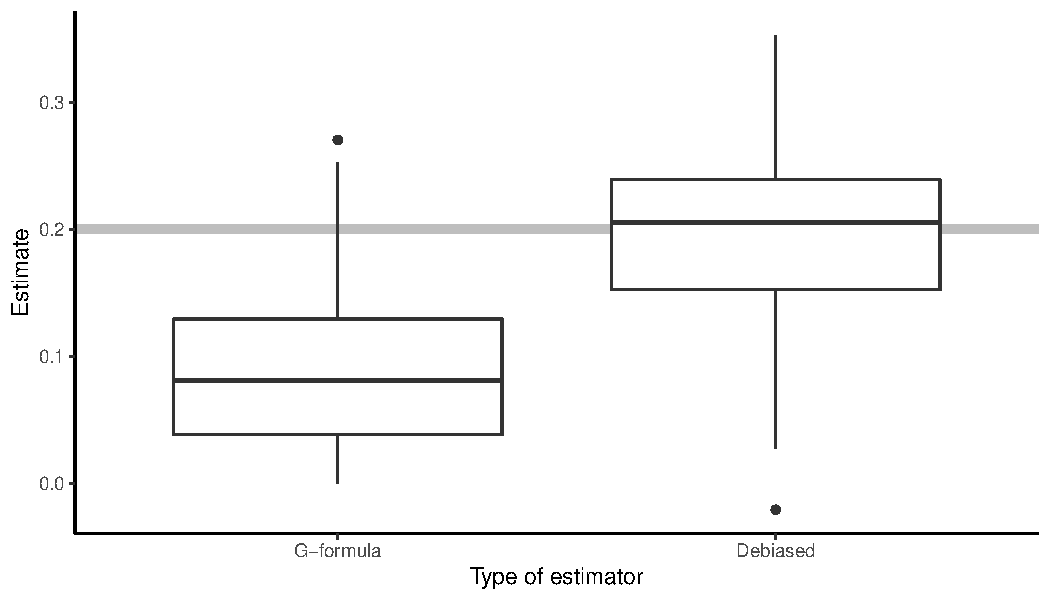
\includegraphics[width=.9\linewidth]{fig-debiased-estimator.pdf}
\end{center}
\end{frame}

\begin{frame}[label={sec:org306328f}]{For the rest of the project}
We now have a zoo of estimators for both the prediction problem and for estimating the ATE:
\begin{enumerate}
\item For the prediction problem:
\begin{itemize}
\item The family of nuisance estimators indexed by our hyperparameter
\item The choice of loss function and splitting procedure used in the cross-validation
\end{itemize}
\item For estimation of the ATE: 
\begin{itemize}
\item The estimator based on the G-formula
\item The debiased estimator
\item For any choice of estimator of the outcome model (and the propensity model) we have an
estimator of the ATE
\end{itemize}
\end{enumerate}

\vfill

\begin{beamercolorbox}[rounded=true]{gray}
\centering What is the effect of these choices on the two estimation problems?
\end{beamercolorbox}
\end{frame}

\begin{frame}[label={sec:org896dddd}]{References}
\small \bibliography{./latex-settings/default-bib.bib}
\end{frame}
\end{document}